\documentclass[12pt,letterpaper,fleqn]{hmcpset}
\usepackage[margin=1in]{geometry}
\usepackage{graphicx}
\usepackage{amsmath,amssymb}
\usepackage{enumerate}
\usepackage{hyperref}
\usepackage{parskip}
\usepackage{listings}

% Theorems
\usepackage{amsthm}
\renewcommand\qedsymbol{$\blacksquare$}
\makeatletter
\@ifclassloaded{article}{
    \newtheorem{definition}{Definition}[section]
    \newtheorem{example}{Example}[section]
    \newtheorem{theorem}{Theorem}[section]
    \newtheorem{corollary}{Corollary}[theorem]
    \newtheorem{lemma}{Lemma}[theorem]
}{
}
\makeatother

% Random Stuff
\setlength\unitlength{1mm}

\newcommand{\insertfig}[3]{
\begin{figure}[htbp]\begin{center}\begin{picture}(120,90)
\put(0,-5){\includegraphics[width=12cm,height=9cm,clip=]{#1.eps}}\end{picture}\end{center}
\caption{#2}\label{#3}\end{figure}}

\newcommand{\insertxfig}[4]{
\begin{figure}[htbp]
\begin{center}
\leavevmode \centerline{\resizebox{#4\textwidth}{!}{\input
#1.pstex_t}}
\caption{#2} \label{#3}
\end{center}
\end{figure}}

\long\def\comment#1{}

\newcommand\norm[1]{\left\lVert#1\right\rVert}
\DeclareMathOperator*{\argmin}{arg\,min}
\DeclareMathOperator*{\argmax}{arg\,max}

% bb font symbols
\newfont{\bbb}{msbm10 scaled 700}
\newcommand{\CCC}{\mbox{\bbb C}}

\newfont{\bbf}{msbm10 scaled 1100}
\newcommand{\CC}{\mbox{\bbf C}}
\newcommand{\PP}{\mbox{\bbf P}}
\newcommand{\RR}{\mbox{\bbf R}}
\newcommand{\QQ}{\mbox{\bbf Q}}
\newcommand{\ZZ}{\mbox{\bbf Z}}
\renewcommand{\SS}{\mbox{\bbf S}}
\newcommand{\FF}{\mbox{\bbf F}}
\newcommand{\GG}{\mbox{\bbf G}}
\newcommand{\EE}{\mbox{\bbf E}}
\newcommand{\NN}{\mbox{\bbf N}}
\newcommand{\KK}{\mbox{\bbf K}}
\newcommand{\KL}{\mbox{\bbf KL}}

% Vectors
\renewcommand{\aa}{{\bf a}}
\newcommand{\bb}{{\bf b}}
\newcommand{\cc}{{\bf c}}
\newcommand{\dd}{{\bf d}}
\newcommand{\ee}{{\bf e}}
\newcommand{\ff}{{\bf f}}
\renewcommand{\gg}{{\bf g}}
\newcommand{\hh}{{\bf h}}
\newcommand{\ii}{{\bf i}}
\newcommand{\jj}{{\bf j}}
\newcommand{\kk}{{\bf k}}
\renewcommand{\ll}{{\bf l}}
\newcommand{\mm}{{\bf m}}
\newcommand{\nn}{{\bf n}}
\newcommand{\oo}{{\bf o}}
\newcommand{\pp}{{\bf p}}
\newcommand{\qq}{{\bf q}}
\newcommand{\rr}{{\bf r}}
\renewcommand{\ss}{{\bf s}}
\renewcommand{\tt}{{\bf t}}
\newcommand{\uu}{{\bf u}}
\newcommand{\ww}{{\bf w}}
\newcommand{\vv}{{\bf v}}
\newcommand{\xx}{{\bf x}}
\newcommand{\yy}{{\bf y}}
\newcommand{\zz}{{\bf z}}
\newcommand{\0}{{\bf 0}}
\newcommand{\1}{{\bf 1}}

% Matrices
\newcommand{\Ab}{{\bf A}}
\newcommand{\Bb}{{\bf B}}
\newcommand{\Cb}{{\bf C}}
\newcommand{\Db}{{\bf D}}
\newcommand{\Eb}{{\bf E}}
\newcommand{\Fb}{{\bf F}}
\newcommand{\Gb}{{\bf G}}
\newcommand{\Hb}{{\bf H}}
\newcommand{\Ib}{{\bf I}}
\newcommand{\Jb}{{\bf J}}
\newcommand{\Kb}{{\bf K}}
\newcommand{\Lb}{{\bf L}}
\newcommand{\Mb}{{\bf M}}
\newcommand{\Nb}{{\bf N}}
\newcommand{\Ob}{{\bf O}}
\newcommand{\Pb}{{\bf P}}
\newcommand{\Qb}{{\bf Q}}
\newcommand{\Rb}{{\bf R}}
\newcommand{\Sb}{{\bf S}}
\newcommand{\Tb}{{\bf T}}
\newcommand{\Ub}{{\bf U}}
\newcommand{\Wb}{{\bf W}}
\newcommand{\Vb}{{\bf V}}
\newcommand{\Xb}{{\bf X}}
\newcommand{\Yb}{{\bf Y}}
\newcommand{\Zb}{{\bf Z}}

% Calligraphic
\newcommand{\Ac}{{\cal A}}
\newcommand{\Bc}{{\cal B}}
\newcommand{\Cc}{{\cal C}}
\newcommand{\Dc}{{\cal D}}
\newcommand{\Ec}{{\cal E}}
\newcommand{\Fc}{{\cal F}}
\newcommand{\Gc}{{\cal G}}
\newcommand{\Hc}{{\cal H}}
\newcommand{\Ic}{{\cal I}}
\newcommand{\Jc}{{\cal J}}
\newcommand{\Kc}{{\cal K}}
\newcommand{\Lc}{{\cal L}}
\newcommand{\Mc}{{\cal M}}
\newcommand{\Nc}{{\cal N}}
\newcommand{\Oc}{{\cal O}}
\newcommand{\Pc}{{\cal P}}
\newcommand{\Qc}{{\cal Q}}
\newcommand{\Rc}{{\cal R}}
\newcommand{\Sc}{{\cal S}}
\newcommand{\Tc}{{\cal T}}
\newcommand{\Uc}{{\cal U}}
\newcommand{\Wc}{{\cal W}}
\newcommand{\Vc}{{\cal V}}
\newcommand{\Xc}{{\cal X}}
\newcommand{\Yc}{{\cal Y}}
\newcommand{\Zc}{{\cal Z}}

% Bold greek letters
\newcommand{\alphab}{\hbox{\boldmath$\alpha$}}
\newcommand{\betab}{\hbox{\boldmath$\beta$}}
\newcommand{\gammab}{\hbox{\boldmath$\gamma$}}
\newcommand{\deltab}{\hbox{\boldmath$\delta$}}
\newcommand{\etab}{\hbox{\boldmath$\eta$}}
\newcommand{\lambdab}{\hbox{\boldmath$\lambda$}}
\newcommand{\epsilonb}{\hbox{\boldmath$\epsilon$}}
\newcommand{\nub}{\hbox{\boldmath$\nu$}}
\newcommand{\mub}{\hbox{\boldmath$\mu$}}
\newcommand{\zetab}{\hbox{\boldmath$\zeta$}}
\newcommand{\phib}{\hbox{\boldmath$\phi$}}
\newcommand{\psib}{\hbox{\boldmath$\psi$}}
\newcommand{\thetab}{\hbox{\boldmath$\theta$}}
\newcommand{\taub}{\hbox{\boldmath$\tau$}}
\newcommand{\omegab}{\hbox{\boldmath$\omega$}}
\newcommand{\xib}{\hbox{\boldmath$\xi$}}
\newcommand{\sigmab}{\hbox{\boldmath$\sigma$}}
\newcommand{\pib}{\hbox{\boldmath$\pi$}}
\newcommand{\rhob}{\hbox{\boldmath$\rho$}}

\newcommand{\Gammab}{\hbox{\boldmath$\Gamma$}}
\newcommand{\Lambdab}{\hbox{\boldmath$\Lambda$}}
\newcommand{\Deltab}{\hbox{\boldmath$\Delta$}}
\newcommand{\Sigmab}{\hbox{\boldmath$\Sigma$}}
\newcommand{\Phib}{\hbox{\boldmath$\Phi$}}
\newcommand{\Pib}{\hbox{\boldmath$\Pi$}}
\newcommand{\Psib}{\hbox{\boldmath$\Psi$}}
\newcommand{\Thetab}{\hbox{\boldmath$\Theta$}}
\newcommand{\Omegab}{\hbox{\boldmath$\Omega$}}
\newcommand{\Xib}{\hbox{\boldmath$\Xi$}}

% mixed symbols
\newcommand{\sinc}{{\hbox{sinc}}}
\newcommand{\diag}{{\hbox{diag}}}
\renewcommand{\det}{{\hbox{det}}}
\newcommand{\trace}{{\hbox{tr}}}
\newcommand{\tr}{\trace}
\newcommand{\sign}{{\hbox{sign}}}
\renewcommand{\arg}{{\hbox{arg}}}
\newcommand{\var}{{\hbox{var}}}
\newcommand{\cov}{{\hbox{cov}}}
\renewcommand{\Re}{{\rm Re}}
\renewcommand{\Im}{{\rm Im}}
\newcommand{\eqdef}{\stackrel{\Delta}{=}}
\newcommand{\defines}{{\,\,\stackrel{\scriptscriptstyle \bigtriangleup}{=}\,\,}}
\newcommand{\<}{\left\langle}
\renewcommand{\>}{\right\rangle}
\newcommand{\Psf}{{\sf P}}
\newcommand{\T}{\top}
\newcommand{\m}[1]{\begin{bmatrix} #1 \end{bmatrix}}

% info for header block in upper right hand corner
\name{Nate Diamant}
\class{Math 189r}
\assignment{Homework 4}
\duedate{November 21, 2016}

\begin{document}

There are 5 problems in this set. You need to do 3 problems the first week and 2 the second
week. Instead of a sixth problem, \textbf{you are encouraged to work on your final project}.
Feel free to work with other students, but make sure you write up the homework
and code on your own (no copying homework \textit{or} code; no pair programming).
Feel free to ask students or instructors for help debugging code or whatever else,
though.
When implementing algorithms you may not use any library (such as \texttt{sklearn})
that already implements the algorithms but you may use any other library for
data cleaning and numeric purposes (\texttt{numpy} or \texttt{pandas}). Use common
sense. Problems are in no specific order.\\[1em]

\textbf{1 (Gaussian Mixture Model)} Consider the generative process for a Gaussian
Mixture Model:
\begin{enumerate}[(1)]
    \item Draw $z_i \sim \mathrm{Cat}(\pib)$ for $i=1,2,\dots,n$.
    \item Draw $\xx_i \sim \Nc(\mub_{z_i}, \Sigmab_{z_i})$ for $i=1,2,\dots,n$.
\end{enumerate}
Note that $z_i$ is unobserved but $\xx_i$ is observed.
Express this model as a directed graphical model, first `unrolled' and then using
Plate notation, before answering the following questions. Support all claims.
\begin{enumerate}[(a)]
    \item Is $\pib$ independent of $\mub_{z_i}$ or $\Sigmab_{z_i}$ given
        your dataset $\Dc = \{\xx_i\}$? Does the posterior distribution over
        $\{\mub,\Sigmab\}$ and $\pib$ factorize? How does this change what inference
        procedure we need to use for this model?
    \item If $z_i$ were observed, would this change? Would the posterior then
        factorize? \textit{Hint:} what other model have we studied that corresponds to
        observing $z_i$?
    \item Find the maximum likelihood estimates for $\pib$, $\mub_k$, and $\Sigmab_k$
        \textit{if} the latent variables $z_i$ were observed.\\

\begin{solution}

    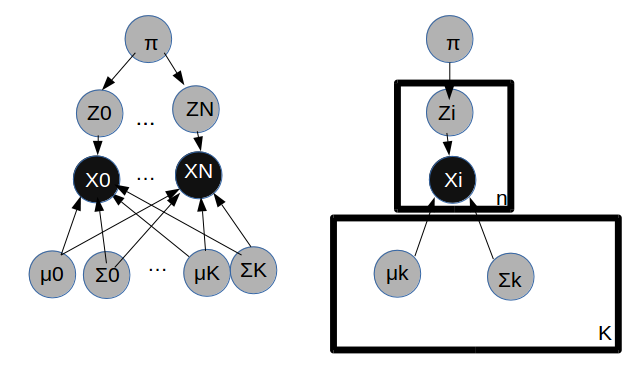
\includegraphics[scale = .5]{p1.png}
    \begin{enumerate}[(a)]
        \item 
            Looking at our DGM, $\pib$ and $\mub_{z_i}$ and $\Sigmab_{z_i}$ are mutually dependent given the data using the Bayes ball algorithm (example c) Murphy 325). The posterior does not factorize, hence the need for the EM algorithm in mixture models.
        \item 
            When $z_i$ are observed, the model becomes Gaussian Discriminant Analysis. The shaded $z_i$ stop the balls from establishing dependence (example a) Murphy 325) The posterior of GDA does factorize, hence the closed form solutions for the variations of GDA.
        \item
            Because $z_i$ are observed, the MLE for $\pib$ is $\pib_k = \frac{1}{n}\sum_i I(z_i = k)$. Similarly, $\mub_{z_i}$ and $\Sigmab_{z_i}$ are just the empirical mean and covariances respectively of their clusters.

    \end{enumerate}
\end{solution}
\end{enumerate}
\newpage

\textbf{2 (Linear Regression)} Consider the Bayesian Linear Regression model with
the following generative process:
\begin{enumerate}[(1)]
    \item Draw $\ww \sim \Nc(\0, \mathbf{V}_0)$
    \item Draw $\yy_i \sim \Nc(\ww^\T\xx_i, \sigma^2)$ for $i=1,2,\dots,n$ where $\sigma^2$
        is known.
\end{enumerate}
Express this model as a directed graphical model using Plate notation. Is $\yy_i$
independent of $\ww$? Is $\yy_i$ independent of $\ww$ \textit{given} $\Dc = \{\xx_i\}$? Support
these claims.
\begin{solution}
    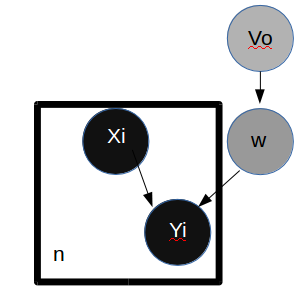
\includegraphics[scale = .5]{p2.png}\\\\
    $\yy_i$ can never be independent of $\ww$ because it is directly formulaicly derived directly from $\ww$.
\end{solution}

\newpage

\textbf{3 (Collaborative Filtering)} Consider the `ratings' matrix $\Rb\in\RR^{n\times n}$
with the low rank approximation $\Rb = \Ub \Vb^\T$ where $\Ub$ and $\Vb$ live in
$\RR^{n\times k}$ where we have $k$ latent factors. Define our optimization problem as
\begin{align*}
    \text{minimize: } & f(\Ub,\Vb) = \|\Rb - \Ub\Vb^\T\|_2^2 + \lambda\|\Ub\|_2^2 + \gamma\|\Vb\|_2^2
\end{align*}
where $\|\cdot\|_2$ in this case is the Frobenius norm $\|\Rb\|_2^2 = \sum_{ij}\Rb_{ij}^2$.
Derive the gradient of $f$ with respect to $\Ub_i$ and $\Vb_j$. Derive a stochastic
approximation to this gradient where you consider a single data point at a time.\\

\begin{solution}
    First we will take the gradient with respect to $\Ub_k$.
    \begin{align*}
        0 &= \nabla_{\Ub_k} \|\Rb - \Ub\Vb^\T\|_2^2 + \lambda\|\Ub\|_2^2 + \gamma\|\Vb\|_2^2\\
        &= \nabla_{\Ub_k} \sum_{ij}(\Rb_{ij} + (\Ub \Vb^\T)_{ij} )^2 - \lambda \sum_{ij} \Ub_{ij}^2 \\
        &= \nabla_{\Ub_k} \sum_{ij}(\Rb_{ij} - \Ub_i \Vb^\T_j )^2 + \lambda \sum_{i} \Ub_i \Ub_i^\T \\
        &=  -2 \sum_{i}(\Rb_{ik} - \Ub_i \Vb^\T_k) \Vb_k - 2\lambda \Ub_{k}
    \end{align*}
    Using the similarity of the problem, 
    $$
        \nabla_{\Vb_k} f(\Ub,\Vb) = -2 \sum_{j}(\Rb_{ik} - \Ub_k \Vb^\T_j) \Ub_k - 2\lambda \Vb_{k}
    $$
    Our stochastic method will only use one data point at a time, so we will drop the sums, yielding,
    \begin{align*}
        & -2 (\Rb_{ik} - \Ub_i \Vb^\T_k) \Vb_k - 2\lambda \Ub_{k} \\
        &  -2 (\Rb_{ik} - \Ub_k \Vb^\T_j) \Ub_k - 2\lambda \Vb_{k}
    \end{align*}
\end{solution}

\newpage

\textbf{4 (Alternating Least Squares)} Consider the same setup and objective
\begin{align*}
    \text{minimize: } & f(\Ub,\Vb) = \|\Rb - \Ub\Vb^\T\|_2^2 + \lambda\|\Ub\|_2^2 + \gamma\|\Vb\|_2^2
\end{align*}
as above in problem (3).
\begin{enumerate}[(a)]
    \item Suppose we fix $\Ub$. Find the optimal $\Vb$.
    \item Suppose we fix $\Vb$. Find the optimal $\Ub$.
    \item Propose an EM-like (block coordinate ascent, to be exact) like algorithm
        for minimizing $f(\Ub,\Vb)$ using (a) and (b).
    \item Will the algorithm you propose in (c) necessarily converge to the global
        optimal?
\end{enumerate}

\begin{solution}
    \begin{enumerate}[(a)]
        \item
            We take the partial with respect to the entire matrix and set it to zero. 
            \begin{align*}
                0 &= \frac{\partial}{\partial \Vb^\T} \|\Rb - \Ub\Vb^\T\|_2^2 + \lambda\|\Ub\|_2^2 + \gamma\|\Vb\|_2^2 \\
                &= \frac{\partial}{\partial \Vb^\T} \|\Rb - \Ub \Vb^\T  \|_2^2 + \lambda\|\Ub\|_2^2 + \gamma\|\Vb^\T \|_2^2 \text{ Transpose of scalar} \\
                &= -2\Ub^\T(\Rb - \Ub\Vb^\T) + 2\gamma \Vb^\T \text{ Matrix Cookbook partial of Frobenius norm} \\
                \Ub^\T \Rb &= (\gamma \Ib  + \Ub^\T \Ub) \Vb^\T  \\
                \Vb^\T &= (\gamma \Ib  + \Ub^\T \Ub)^{-1} \Ub^\T \Rb
            \end{align*}
        \item
            Similarly,
            \begin{align*}
                0 &= \frac{\partial}{\partial \Ub} \|\Rb - \Ub\Vb^\T\|_2^2 + \lambda\|\Ub\|_2^2 + \gamma\|\Vb\|_2^2 \\
                &= -2 (\Rb - \Ub\Vb^\T) \Vb + 2 \lambda \Ub \\
                \Rb \Vb &= \Ub (\Vb^\T \Vb + \lambda \Ib) \\
                \Ub &= \Rb \Vb(\Vb^\T \Vb + \lambda \Ib)^{-1}
            \end{align*}
        \item
            My algorithm starts with some guessed $\Ub$. Using that, it then calculates the optimal $\Vb^\T$ using the closed form above. With that $\Vb^\T$, calculate the optimal $\Ub$. Repeat until the cost function is less than some specified precision.
        \item
            Consider the single variate case:
            $$
                (R-UV)^2 + \lambda U^2 + \gamma V^2\\       
            $$
            The Hessian with $R, V$ as variables is (Mathematica):
            $$\left(
                \begin{array}{cc}
                 2 V^2+2 \lambda  & 2 U V-2 (R-U V) \\
                 2 U V-2 (R-U V) & 2 U^2+2 \gamma  \\
                \end{array}
            \right)$$
            which is not necessarily positive definite.


    \end{enumerate}
\end{solution}

\textbf{5 (Non-Negative Matrix Factorization)} Consider the dataset at
\url{http://kdd.ics.uci.edu/databases/reuters21578/reuters21578.html}. Choosing an appropriate
objective function and algorithm from Lee and Seung 2001\footnote{\url{https://papers.nips.cc/paper/1861-algorithms-for-non-negative-matrix-factorization.pdf}}
implement Non-Negative Matrix Factorization for topic modelling (choose an appropriate number
of topics/latent features) and assert that the convergence properties proved in the paper hold. 
Display the 20 most relevant words for each of the topics you discover.

\end{document}
